% Single laser work
\documentclass[10pt,twocolumn,letterpaper]{article}

\usepackage[pdftex]{graphicx} % for \includegraphics[scale=•]{•}
\usepackage{color}
\usepackage{pgf}


\begin{document}
\title{[DRAFT] - Stage Oriented Design of an Intersection Management System Based on Laser Scanner Data}

\author{Gustavo Velasco-Hernandez, Eduardo Caicedo-Bravo \\
Universidad del Valle\\
{\tt\small velasco.gustavo@correounivalle.edu.co, eduardo.caicedo@correounivalle.edu.co}
% For a paper whose authors are all at the same institution,
% omit the following lines up until the closing ``}''.
% Additional authors and addresses can be added with ``\and'',
% just like the second author.
% To save space, use either the email address or home page, not both
}

\maketitle

\begin{abstract}
The supervision of vehicular intersections is a major need for improving transportation systems because these are complex scenarios where different traffic elements interact between them. Recently, laser-based systems have been proposed and implemented to sense and to monitor intersections, giving good results as those based on cameras. In this work a stage-oriented design of an intersection management system based on laserscanner sensor data is proposed. The main objective of the proposed architecture is that it should have scalability, modularity, and high integrability. In order to achieve those objectives, the process flow of an intersection management system (IMS) is divided into four stages: preprocessing, feature analysis, pattern recognition, and situation assessment. Each of these stages is explained and some commonly used techniques are described. Finally, we present an example implementation using a laserscanner dataset, both in a single-laser approach and a multi-laser approach.

\end{abstract}


\section{Introduction}

In transportation systems one of the most desirable scenarios to improve efficiency and safety are intersections. This because intersections are places where vehicles arrive from different directions at different velocities, increasing the chances for incidents and crashes. Choi \cite{Choi2010} states that 40\% of reported traffic accidents in the US, were intersection related. Also, in  \cite{CorporacionFondodePrevencionVial2010}, is reported that for Colombia in 2011, most of the accidents in the main cities were at intersections.

Several approaches for monitoring intersections are based on sensors on infrastructure like inductive loops, range scanners and cameras. Inductive loops detects presence of vehicles, which is simple for processing but information that could be extracted from they is limited. Cameras, on the other side, offer a high volume of data, but their processing requirements are high for extracting information. Range scanners are an intermediate option in which data from them is much high than from inductive loops, but not as high as from cameras and processing techniques for range data are not computational expensive as those for treating images or videos.

\begin{figure}[ht!]
\centering
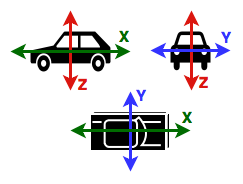
\includegraphics[scale=0.8]{fig/carReferenceSystem.png}
\caption{Vehicle reference coordinate system}
\label{vehicle_cs}
\end{figure}

For range-based traffic monitoring systems there are three commonly used reference coordinate system for vehicles (Figure \ref{vehicle_cs}). Based on this, several laser-based systems have been proposed taking a plane as the main plane for laser scanner positioning. For example, F{\"u}erstenberg in  \cite{Fuerstenberg2000} proposes the use XZ plane scanning for vehicle classification and scanning on YZ plane for vehicle counting. Related to YZ plane, \cite{Harlow2001} and \cite{Vivet2013} present a deployment for vehicle monitoring scanning from the top and Gómez in \cite{Gomez2013} presents a side-view scanning for vehicle classification fused with a vision system. In \cite{Goldhammer2012} and \cite{Strigel2014}, Goldhammer and Striegel, respectively, detail an implemetation using a set of multilayer laser scanners deployed in different configurations for scanning from the top of the road, some using YZ plane and some using XZ plane. Recently, the use of XY plane has increased, and two main approaches arise: on-road and on-board systems. On-road systems are installed in infrastructure, aiming to detect passing vehicles, while on-board systems are installed on vehicles to detect the sourrounding environment. Both of them take the XY plane as main plane for scanning. Some examples of on-road sytems could be found in \cite{Zhao2006, Zhao2008, Zhao2009, Zhao2012} and \cite{Perng2014}. Petrovskaya in \cite{Petrovskaya2009} presents an On-board implementation.

All of the previous developments share a common processing stages that could be enumarated: preprocessing, feature analysis, pattern recognition, and situation assessment. In the section 2, these stages are explained and some common processing substages for each one are introduced. In section 3 is presented an example implementation based on a dataset and showing some methods and techniques used in the proposed stages. Section 4 presents the result of a single-laser and a multi-laser deployments. Finally, in section 6 are summarized the conclusions and some future work perspectives are proposed.



\section{Stages Definition}
In the designing of an IMS, there are four main stages that have to be performed from the data source to final output: preprocessing, feature analysis, pattern recognition and situation assessment.

The aim of the first stage is to extract data of interest from the raw sensor information, using filtering and background subtraction techniques to get the foreground of the scene, remove noise and irrelevant data. Spatio-temporal alignment of data is also performed in this stage. In the second stage, the objective is to identify elements within the foreground and extract relevant features of them. The third stage receives the set of features from the previous stage and performs recognition and classification tasks. Also, tracking and prediction of objects' state is performed based on historic information. In the fourth stage, object behaviour and inter-objects interaction are analysed to identify context and detect situation or events of interest.

The output of the fourth stage could be delivered to an optional fifth stage of decision and control, to a human operator, or to a traffic agent or institution, to take immediate actions on traffic control, issue traffic tickets, warn drivers about possible incidents or improve transportation policies in a long-term basis. In figure \ref{proc_stages}, previously described stages are depicted, and also is shown how the data volume is reduced while data meaning increases in the last stages.

\begin{figure}[ht!]
\centering
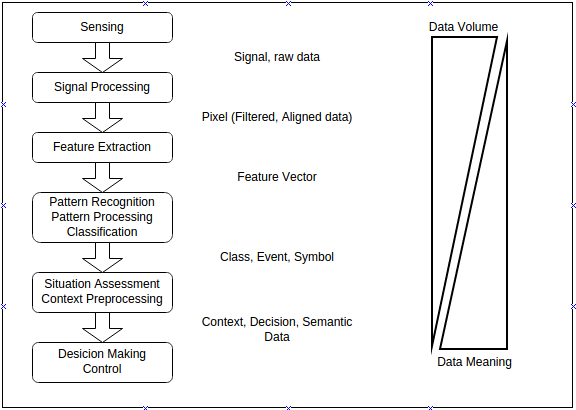
\includegraphics[scale=0.35]{../fig/3/proc_stages.png}
\caption{Dataflow through processing stages in an IMS.}
\label{proc_stages}
\end{figure}

Different tasks could be performed in each aforementioned stages, as is referred in figure \ref{proc_stages_tasks}. Below there is a description of common concepts and techniques associated with each of these tasks.

\begin{figure}[ht!]
\centering
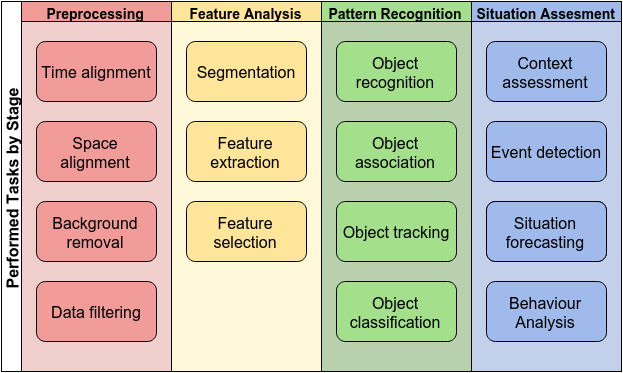
\includegraphics[scale=0.35]{../fig/3/processing_stages_and_tasks.png}
\caption{Processing stages and tasks performed.}
\label{proc_stages_tasks}
\end{figure}
\subsection{Preprocessing}

 In the preprocessing stage raw data from sensor is received and the purpose is to enhance this data through filtering, removing noise and discarding corrupted data. Also, space and time alignment is done in this stage.

\subsubsection{Background Removing}
 
In order to extract meaningful information, background removal techniques are applied in this stage. For doing this, a background model should be generated. One typical approach to generate a background model is to use a threshold to determine if certain measure corresponds to background or foreground. This threshold is computed based on a peak value found in histogram of the measure within a time window. Another approach consist in describe the data using a probability distribution function, using maximum likelihood estimation, commonly of a gaussian model.
 
Sometimes, the threshold technique is enough for modeling static backgrounds like walls, buildings or ground. But in other cases, it could be found a non-stable background, for example, when there exist moving vegetation or object borders, and a mixture of models may retrieve a better representation of the data instead.

\subsubsection{Space and Time alignment}

In some cases, it could be desired to have a fixed base of time for trigger sensor readings, for synchronisation purposes or for implement fusion between different sensors within a time slot. It is for this reason that time alignment of data is done.

On the other side, in the case of laser scanners, the measures are referenced to its own coordinate systems. Calibration is needed to transform those measures to a global coordinate systems which represents the whole intersection scenario. 

\subsection{Feature Analysis}

After obtaining the foreground of the scene, it is needed to extract relevant points that could represent elements of interest in the intersection, like vehicles, pedestrians or obstacles. In this stage clustering is used to group points that belong to the same object, and for the nature of the environment, algorithms where estimated number of cluster is not needed are prefered. 


\subsection{Pattern Recognition}

From the previous stage we have a set of blobs as result of clustering, and based on the features of those blobs, different classes of objects could be recognized. Different classification types are implemented depending on the type of application, binary classification or multiclass classification.

When objects are identified, some relations between objects should be extracted to get more information about the scene. Relations between objects of the same class, objects of different classes or objects and environment are possible, both in a single timeslot or in sucesive timeslots. 

\subsection{Situation Assesment}

-TODO-

\section{Laser-based System Implementation}

\subsection{Dataset}
 The dataset used for this work was provided by POSS research group and was used for \cite{Zhao2009}. The dataset consist of ten minutes of laser scanner raw data from six sensors arranged horizontally over an intersection near Peking University. Background model and calibration data for each laser scanner is also provided. Additionally, dataset contains trajectory info of objects in the scene, generated by their algorithm. Figure \ref{inter_cfg} show intersection scenario, indicating position and orientation of each laser scanner inlcuded in dataset.

\begin{figure}
    \centering
    %% Creator: Matplotlib, PGF backend
%%
%% To include the figure in your LaTeX document, write
%%   \input{<filename>.pgf}
%%
%% Make sure the required packages are loaded in your preamble
%%   \usepackage{pgf}
%%
%% Figures using additional raster images can only be included by \input if
%% they are in the same directory as the main LaTeX file. For loading figures
%% from other directories you can use the `import` package
%%   \usepackage{import}
%% and then include the figures with
%%   \import{<path to file>}{<filename>.pgf}
%%
%% Matplotlib used the following preamble
%%   \usepackage[utf8x]{inputenc}
%%   \usepackage[T1]{fontenc}
%%
\begingroup%
\makeatletter%
\begin{pgfpicture}%
\pgfpathrectangle{\pgfpointorigin}{\pgfqpoint{3.000000in}{2.250000in}}%
\pgfusepath{use as bounding box, clip}%
\begin{pgfscope}%
\pgfsetbuttcap%
\pgfsetmiterjoin%
\definecolor{currentfill}{rgb}{1.000000,1.000000,1.000000}%
\pgfsetfillcolor{currentfill}%
\pgfsetlinewidth{0.000000pt}%
\definecolor{currentstroke}{rgb}{1.000000,1.000000,1.000000}%
\pgfsetstrokecolor{currentstroke}%
\pgfsetdash{}{0pt}%
\pgfpathmoveto{\pgfqpoint{0.000000in}{0.000000in}}%
\pgfpathlineto{\pgfqpoint{3.000000in}{0.000000in}}%
\pgfpathlineto{\pgfqpoint{3.000000in}{2.250000in}}%
\pgfpathlineto{\pgfqpoint{0.000000in}{2.250000in}}%
\pgfpathclose%
\pgfusepath{fill}%
\end{pgfscope}%
\begin{pgfscope}%
\pgfsetbuttcap%
\pgfsetmiterjoin%
\definecolor{currentfill}{rgb}{1.000000,1.000000,1.000000}%
\pgfsetfillcolor{currentfill}%
\pgfsetlinewidth{0.000000pt}%
\definecolor{currentstroke}{rgb}{0.000000,0.000000,0.000000}%
\pgfsetstrokecolor{currentstroke}%
\pgfsetstrokeopacity{0.000000}%
\pgfsetdash{}{0pt}%
\pgfpathmoveto{\pgfqpoint{0.375000in}{0.225000in}}%
\pgfpathlineto{\pgfqpoint{2.700000in}{0.225000in}}%
\pgfpathlineto{\pgfqpoint{2.700000in}{2.025000in}}%
\pgfpathlineto{\pgfqpoint{0.375000in}{2.025000in}}%
\pgfpathclose%
\pgfusepath{fill}%
\end{pgfscope}%
\begin{pgfscope}%
\pgfpathrectangle{\pgfqpoint{0.375000in}{0.225000in}}{\pgfqpoint{2.325000in}{1.800000in}} %
\pgfusepath{clip}%
\pgftext[at=\pgfqpoint{0.375000in}{0.225000in},left,bottom]{\pgfimage[interpolate=true,width=2.330000in,height=1.810000in]{intersection-config2-img0.png}}%
\end{pgfscope}%
\begin{pgfscope}%
\pgfpathrectangle{\pgfqpoint{0.375000in}{0.225000in}}{\pgfqpoint{2.325000in}{1.800000in}} %
\pgfusepath{clip}%
\pgfsetbuttcap%
\pgfsetmiterjoin%
\definecolor{currentfill}{rgb}{0.000000,0.000000,1.000000}%
\pgfsetfillcolor{currentfill}%
\pgfsetlinewidth{1.003750pt}%
\definecolor{currentstroke}{rgb}{0.000000,0.000000,1.000000}%
\pgfsetstrokecolor{currentstroke}%
\pgfsetdash{}{0pt}%
\pgfpathmoveto{\pgfqpoint{1.333175in}{0.309514in}}%
\pgfpathlineto{\pgfqpoint{1.352184in}{0.312481in}}%
\pgfpathlineto{\pgfqpoint{1.342601in}{0.377890in}}%
\pgfpathlineto{\pgfqpoint{1.361611in}{0.380857in}}%
\pgfpathlineto{\pgfqpoint{1.330701in}{0.392758in}}%
\pgfpathlineto{\pgfqpoint{1.304583in}{0.371954in}}%
\pgfpathlineto{\pgfqpoint{1.323592in}{0.374922in}}%
\pgfpathclose%
\pgfusepath{stroke,fill}%
\end{pgfscope}%
\begin{pgfscope}%
\pgfpathrectangle{\pgfqpoint{0.375000in}{0.225000in}}{\pgfqpoint{2.325000in}{1.800000in}} %
\pgfusepath{clip}%
\pgfsetbuttcap%
\pgfsetmiterjoin%
\definecolor{currentfill}{rgb}{0.000000,0.000000,1.000000}%
\pgfsetfillcolor{currentfill}%
\pgfsetlinewidth{1.003750pt}%
\definecolor{currentstroke}{rgb}{0.000000,0.000000,1.000000}%
\pgfsetstrokecolor{currentstroke}%
\pgfsetdash{}{0pt}%
\pgfpathmoveto{\pgfqpoint{2.111500in}{1.532814in}}%
\pgfpathlineto{\pgfqpoint{2.092668in}{1.536805in}}%
\pgfpathlineto{\pgfqpoint{2.079782in}{1.472004in}}%
\pgfpathlineto{\pgfqpoint{2.060949in}{1.475995in}}%
\pgfpathlineto{\pgfqpoint{2.085976in}{1.453809in}}%
\pgfpathlineto{\pgfqpoint{2.117447in}{1.464023in}}%
\pgfpathlineto{\pgfqpoint{2.098614in}{1.468013in}}%
\pgfpathclose%
\pgfusepath{stroke,fill}%
\end{pgfscope}%
\begin{pgfscope}%
\pgfpathrectangle{\pgfqpoint{0.375000in}{0.225000in}}{\pgfqpoint{2.325000in}{1.800000in}} %
\pgfusepath{clip}%
\pgfsetbuttcap%
\pgfsetmiterjoin%
\definecolor{currentfill}{rgb}{0.000000,0.000000,1.000000}%
\pgfsetfillcolor{currentfill}%
\pgfsetlinewidth{1.003750pt}%
\definecolor{currentstroke}{rgb}{0.000000,0.000000,1.000000}%
\pgfsetstrokecolor{currentstroke}%
\pgfsetdash{}{0pt}%
\pgfpathmoveto{\pgfqpoint{1.767998in}{1.893430in}}%
\pgfpathlineto{\pgfqpoint{1.758154in}{1.910476in}}%
\pgfpathlineto{\pgfqpoint{1.703107in}{1.876604in}}%
\pgfpathlineto{\pgfqpoint{1.693263in}{1.893650in}}%
\pgfpathlineto{\pgfqpoint{1.694268in}{1.859612in}}%
\pgfpathlineto{\pgfqpoint{1.722796in}{1.842511in}}%
\pgfpathlineto{\pgfqpoint{1.712952in}{1.859557in}}%
\pgfpathclose%
\pgfusepath{stroke,fill}%
\end{pgfscope}%
\begin{pgfscope}%
\pgfpathrectangle{\pgfqpoint{0.375000in}{0.225000in}}{\pgfqpoint{2.325000in}{1.800000in}} %
\pgfusepath{clip}%
\pgfsetbuttcap%
\pgfsetmiterjoin%
\definecolor{currentfill}{rgb}{0.000000,0.000000,1.000000}%
\pgfsetfillcolor{currentfill}%
\pgfsetlinewidth{1.003750pt}%
\definecolor{currentstroke}{rgb}{0.000000,0.000000,1.000000}%
\pgfsetstrokecolor{currentstroke}%
\pgfsetdash{}{0pt}%
\pgfpathmoveto{\pgfqpoint{1.739381in}{0.300340in}}%
\pgfpathlineto{\pgfqpoint{1.758573in}{0.299163in}}%
\pgfpathlineto{\pgfqpoint{1.762373in}{0.365199in}}%
\pgfpathlineto{\pgfqpoint{1.781565in}{0.364022in}}%
\pgfpathlineto{\pgfqpoint{1.753728in}{0.382296in}}%
\pgfpathlineto{\pgfqpoint{1.723990in}{0.367553in}}%
\pgfpathlineto{\pgfqpoint{1.743182in}{0.366376in}}%
\pgfpathclose%
\pgfusepath{stroke,fill}%
\end{pgfscope}%
\begin{pgfscope}%
\pgfpathrectangle{\pgfqpoint{0.375000in}{0.225000in}}{\pgfqpoint{2.325000in}{1.800000in}} %
\pgfusepath{clip}%
\pgfsetbuttcap%
\pgfsetmiterjoin%
\definecolor{currentfill}{rgb}{0.000000,0.000000,1.000000}%
\pgfsetfillcolor{currentfill}%
\pgfsetlinewidth{1.003750pt}%
\definecolor{currentstroke}{rgb}{0.000000,0.000000,1.000000}%
\pgfsetstrokecolor{currentstroke}%
\pgfsetdash{}{0pt}%
\pgfpathmoveto{\pgfqpoint{1.086267in}{1.589504in}}%
\pgfpathlineto{\pgfqpoint{1.069753in}{1.579343in}}%
\pgfpathlineto{\pgfqpoint{1.102567in}{1.522521in}}%
\pgfpathlineto{\pgfqpoint{1.086053in}{1.512359in}}%
\pgfpathlineto{\pgfqpoint{1.119027in}{1.513396in}}%
\pgfpathlineto{\pgfqpoint{1.135595in}{1.542844in}}%
\pgfpathlineto{\pgfqpoint{1.119081in}{1.532683in}}%
\pgfpathclose%
\pgfusepath{stroke,fill}%
\end{pgfscope}%
\begin{pgfscope}%
\pgfpathrectangle{\pgfqpoint{0.375000in}{0.225000in}}{\pgfqpoint{2.325000in}{1.800000in}} %
\pgfusepath{clip}%
\pgfsetbuttcap%
\pgfsetmiterjoin%
\definecolor{currentfill}{rgb}{0.000000,0.000000,1.000000}%
\pgfsetfillcolor{currentfill}%
\pgfsetlinewidth{1.003750pt}%
\definecolor{currentstroke}{rgb}{0.000000,0.000000,1.000000}%
\pgfsetstrokecolor{currentstroke}%
\pgfsetdash{}{0pt}%
\pgfpathmoveto{\pgfqpoint{1.275600in}{1.774295in}}%
\pgfpathlineto{\pgfqpoint{1.268773in}{1.755742in}}%
\pgfpathlineto{\pgfqpoint{1.328681in}{1.732251in}}%
\pgfpathlineto{\pgfqpoint{1.321854in}{1.713699in}}%
\pgfpathlineto{\pgfqpoint{1.347072in}{1.735655in}}%
\pgfpathlineto{\pgfqpoint{1.342335in}{1.769356in}}%
\pgfpathlineto{\pgfqpoint{1.335508in}{1.750804in}}%
\pgfpathclose%
\pgfusepath{stroke,fill}%
\end{pgfscope}%
\begin{pgfscope}%
\pgfpathrectangle{\pgfqpoint{0.375000in}{0.225000in}}{\pgfqpoint{2.325000in}{1.800000in}} %
\pgfusepath{clip}%
\pgfsetbuttcap%
\pgfsetmiterjoin%
\pgfsetlinewidth{2.007500pt}%
\definecolor{currentstroke}{rgb}{0.000000,0.501961,0.000000}%
\pgfsetstrokecolor{currentstroke}%
\pgfsetdash{}{0pt}%
\pgfpathmoveto{\pgfqpoint{1.557364in}{1.514964in}}%
\pgfpathlineto{\pgfqpoint{1.743209in}{1.514964in}}%
\pgfpathlineto{\pgfqpoint{1.743209in}{2.027642in}}%
\pgfpathlineto{\pgfqpoint{1.557364in}{2.027642in}}%
\pgfpathlineto{\pgfqpoint{1.557364in}{1.514964in}}%
\pgfpathclose%
\pgfusepath{stroke}%
\end{pgfscope}%
\begin{pgfscope}%
\pgfpathrectangle{\pgfqpoint{0.375000in}{0.225000in}}{\pgfqpoint{2.325000in}{1.800000in}} %
\pgfusepath{clip}%
\pgfsetbuttcap%
\pgfsetmiterjoin%
\pgfsetlinewidth{2.007500pt}%
\definecolor{currentstroke}{rgb}{1.000000,0.000000,0.000000}%
\pgfsetstrokecolor{currentstroke}%
\pgfsetdash{}{0pt}%
\pgfpathmoveto{\pgfqpoint{1.919442in}{1.099860in}}%
\pgfpathlineto{\pgfqpoint{2.419304in}{1.099860in}}%
\pgfpathlineto{\pgfqpoint{2.419304in}{1.465350in}}%
\pgfpathlineto{\pgfqpoint{1.919442in}{1.465350in}}%
\pgfpathlineto{\pgfqpoint{1.919442in}{1.099860in}}%
\pgfpathclose%
\pgfusepath{stroke}%
\end{pgfscope}%
\begin{pgfscope}%
\pgfpathrectangle{\pgfqpoint{0.375000in}{0.225000in}}{\pgfqpoint{2.325000in}{1.800000in}} %
\pgfusepath{clip}%
\pgfsetbuttcap%
\pgfsetmiterjoin%
\pgfsetlinewidth{2.007500pt}%
\definecolor{currentstroke}{rgb}{0.000000,0.501961,0.000000}%
\pgfsetstrokecolor{currentstroke}%
\pgfsetdash{}{0pt}%
\pgfpathmoveto{\pgfqpoint{1.919442in}{0.380457in}}%
\pgfpathlineto{\pgfqpoint{2.419304in}{0.380457in}}%
\pgfpathlineto{\pgfqpoint{2.419304in}{0.706256in}}%
\pgfpathlineto{\pgfqpoint{1.919442in}{0.706256in}}%
\pgfpathlineto{\pgfqpoint{1.919442in}{0.380457in}}%
\pgfpathclose%
\pgfusepath{stroke}%
\end{pgfscope}%
\begin{pgfscope}%
\pgfpathrectangle{\pgfqpoint{0.375000in}{0.225000in}}{\pgfqpoint{2.325000in}{1.800000in}} %
\pgfusepath{clip}%
\pgfsetbuttcap%
\pgfsetmiterjoin%
\pgfsetlinewidth{2.007500pt}%
\definecolor{currentstroke}{rgb}{1.000000,0.000000,0.000000}%
\pgfsetstrokecolor{currentstroke}%
\pgfsetdash{}{0pt}%
\pgfpathmoveto{\pgfqpoint{0.698628in}{0.380457in}}%
\pgfpathlineto{\pgfqpoint{1.102362in}{0.380457in}}%
\pgfpathlineto{\pgfqpoint{1.102362in}{0.746939in}}%
\pgfpathlineto{\pgfqpoint{0.698628in}{0.746939in}}%
\pgfpathlineto{\pgfqpoint{0.698628in}{0.380457in}}%
\pgfpathclose%
\pgfusepath{stroke}%
\end{pgfscope}%
\begin{pgfscope}%
\pgfpathrectangle{\pgfqpoint{0.375000in}{0.225000in}}{\pgfqpoint{2.325000in}{1.800000in}} %
\pgfusepath{clip}%
\pgfsetbuttcap%
\pgfsetmiterjoin%
\pgfsetlinewidth{2.007500pt}%
\definecolor{currentstroke}{rgb}{0.000000,0.501961,0.000000}%
\pgfsetstrokecolor{currentstroke}%
\pgfsetdash{}{0pt}%
\pgfpathmoveto{\pgfqpoint{0.698628in}{1.129629in}}%
\pgfpathlineto{\pgfqpoint{1.102362in}{1.129629in}}%
\pgfpathlineto{\pgfqpoint{1.102362in}{1.498426in}}%
\pgfpathlineto{\pgfqpoint{0.698628in}{1.498426in}}%
\pgfpathlineto{\pgfqpoint{0.698628in}{1.129629in}}%
\pgfpathclose%
\pgfusepath{stroke}%
\end{pgfscope}%
\begin{pgfscope}%
\pgfpathrectangle{\pgfqpoint{0.375000in}{0.225000in}}{\pgfqpoint{2.325000in}{1.800000in}} %
\pgfusepath{clip}%
\pgfsetbuttcap%
\pgfsetmiterjoin%
\pgfsetlinewidth{2.007500pt}%
\definecolor{currentstroke}{rgb}{1.000000,0.000000,0.000000}%
\pgfsetstrokecolor{currentstroke}%
\pgfsetdash{}{0pt}%
\pgfpathmoveto{\pgfqpoint{1.371518in}{1.514964in}}%
\pgfpathlineto{\pgfqpoint{1.557364in}{1.514964in}}%
\pgfpathlineto{\pgfqpoint{1.557364in}{2.027642in}}%
\pgfpathlineto{\pgfqpoint{1.371518in}{2.027642in}}%
\pgfpathlineto{\pgfqpoint{1.371518in}{1.514964in}}%
\pgfpathclose%
\pgfusepath{stroke}%
\end{pgfscope}%
\begin{pgfscope}%
\pgfpathrectangle{\pgfqpoint{0.375000in}{0.225000in}}{\pgfqpoint{2.325000in}{1.800000in}} %
\pgfusepath{clip}%
\pgfsetbuttcap%
\pgfsetmiterjoin%
\definecolor{currentfill}{rgb}{0.000000,0.501961,0.000000}%
\pgfsetfillcolor{currentfill}%
\pgfsetlinewidth{1.003750pt}%
\definecolor{currentstroke}{rgb}{0.000000,0.501961,0.000000}%
\pgfsetstrokecolor{currentstroke}%
\pgfsetdash{}{0pt}%
\pgfpathmoveto{\pgfqpoint{1.647082in}{1.605923in}}%
\pgfpathlineto{\pgfqpoint{1.659899in}{1.605923in}}%
\pgfpathlineto{\pgfqpoint{1.659899in}{1.738227in}}%
\pgfpathlineto{\pgfqpoint{1.672716in}{1.738227in}}%
\pgfpathlineto{\pgfqpoint{1.653491in}{1.771303in}}%
\pgfpathlineto{\pgfqpoint{1.634265in}{1.738227in}}%
\pgfpathlineto{\pgfqpoint{1.647082in}{1.738227in}}%
\pgfpathclose%
\pgfusepath{stroke,fill}%
\end{pgfscope}%
\begin{pgfscope}%
\pgfpathrectangle{\pgfqpoint{0.375000in}{0.225000in}}{\pgfqpoint{2.325000in}{1.800000in}} %
\pgfusepath{clip}%
\pgfsetbuttcap%
\pgfsetmiterjoin%
\definecolor{currentfill}{rgb}{1.000000,0.000000,0.000000}%
\pgfsetfillcolor{currentfill}%
\pgfsetlinewidth{1.003750pt}%
\definecolor{currentstroke}{rgb}{1.000000,0.000000,0.000000}%
\pgfsetstrokecolor{currentstroke}%
\pgfsetdash{}{0pt}%
\pgfpathmoveto{\pgfqpoint{2.175781in}{1.283432in}}%
\pgfpathlineto{\pgfqpoint{2.175781in}{1.296662in}}%
\pgfpathlineto{\pgfqpoint{2.047612in}{1.296662in}}%
\pgfpathlineto{\pgfqpoint{2.047612in}{1.309893in}}%
\pgfpathlineto{\pgfqpoint{2.015570in}{1.290047in}}%
\pgfpathlineto{\pgfqpoint{2.047612in}{1.270202in}}%
\pgfpathlineto{\pgfqpoint{2.047612in}{1.283432in}}%
\pgfpathclose%
\pgfusepath{stroke,fill}%
\end{pgfscope}%
\begin{pgfscope}%
\pgfpathrectangle{\pgfqpoint{0.375000in}{0.225000in}}{\pgfqpoint{2.325000in}{1.800000in}} %
\pgfusepath{clip}%
\pgfsetbuttcap%
\pgfsetmiterjoin%
\definecolor{currentfill}{rgb}{0.000000,0.501961,0.000000}%
\pgfsetfillcolor{currentfill}%
\pgfsetlinewidth{1.003750pt}%
\definecolor{currentstroke}{rgb}{0.000000,0.501961,0.000000}%
\pgfsetstrokecolor{currentstroke}%
\pgfsetdash{}{0pt}%
\pgfpathmoveto{\pgfqpoint{2.015570in}{0.552452in}}%
\pgfpathlineto{\pgfqpoint{2.015570in}{0.539222in}}%
\pgfpathlineto{\pgfqpoint{2.143739in}{0.539222in}}%
\pgfpathlineto{\pgfqpoint{2.143739in}{0.525992in}}%
\pgfpathlineto{\pgfqpoint{2.175781in}{0.545837in}}%
\pgfpathlineto{\pgfqpoint{2.143739in}{0.565683in}}%
\pgfpathlineto{\pgfqpoint{2.143739in}{0.552452in}}%
\pgfpathclose%
\pgfusepath{stroke,fill}%
\end{pgfscope}%
\begin{pgfscope}%
\pgfpathrectangle{\pgfqpoint{0.375000in}{0.225000in}}{\pgfqpoint{2.325000in}{1.800000in}} %
\pgfusepath{clip}%
\pgfsetbuttcap%
\pgfsetmiterjoin%
\definecolor{currentfill}{rgb}{1.000000,0.000000,0.000000}%
\pgfsetfillcolor{currentfill}%
\pgfsetlinewidth{1.003750pt}%
\definecolor{currentstroke}{rgb}{1.000000,0.000000,0.000000}%
\pgfsetstrokecolor{currentstroke}%
\pgfsetdash{}{0pt}%
\pgfpathmoveto{\pgfqpoint{0.906903in}{0.577259in}}%
\pgfpathlineto{\pgfqpoint{0.906903in}{0.564029in}}%
\pgfpathlineto{\pgfqpoint{1.035073in}{0.564029in}}%
\pgfpathlineto{\pgfqpoint{1.035073in}{0.550799in}}%
\pgfpathlineto{\pgfqpoint{1.067115in}{0.570644in}}%
\pgfpathlineto{\pgfqpoint{1.035073in}{0.590490in}}%
\pgfpathlineto{\pgfqpoint{1.035073in}{0.577259in}}%
\pgfpathclose%
\pgfusepath{stroke,fill}%
\end{pgfscope}%
\begin{pgfscope}%
\pgfpathrectangle{\pgfqpoint{0.375000in}{0.225000in}}{\pgfqpoint{2.325000in}{1.800000in}} %
\pgfusepath{clip}%
\pgfsetbuttcap%
\pgfsetmiterjoin%
\definecolor{currentfill}{rgb}{0.000000,0.501961,0.000000}%
\pgfsetfillcolor{currentfill}%
\pgfsetlinewidth{1.003750pt}%
\definecolor{currentstroke}{rgb}{0.000000,0.501961,0.000000}%
\pgfsetstrokecolor{currentstroke}%
\pgfsetdash{}{0pt}%
\pgfpathmoveto{\pgfqpoint{1.067115in}{1.313200in}}%
\pgfpathlineto{\pgfqpoint{1.067115in}{1.326431in}}%
\pgfpathlineto{\pgfqpoint{0.938946in}{1.326431in}}%
\pgfpathlineto{\pgfqpoint{0.938946in}{1.339661in}}%
\pgfpathlineto{\pgfqpoint{0.906903in}{1.319816in}}%
\pgfpathlineto{\pgfqpoint{0.938946in}{1.299970in}}%
\pgfpathlineto{\pgfqpoint{0.938946in}{1.313200in}}%
\pgfpathclose%
\pgfusepath{stroke,fill}%
\end{pgfscope}%
\begin{pgfscope}%
\pgfpathrectangle{\pgfqpoint{0.375000in}{0.225000in}}{\pgfqpoint{2.325000in}{1.800000in}} %
\pgfusepath{clip}%
\pgfsetbuttcap%
\pgfsetmiterjoin%
\definecolor{currentfill}{rgb}{1.000000,0.000000,0.000000}%
\pgfsetfillcolor{currentfill}%
\pgfsetlinewidth{1.003750pt}%
\definecolor{currentstroke}{rgb}{1.000000,0.000000,0.000000}%
\pgfsetstrokecolor{currentstroke}%
\pgfsetdash{}{0pt}%
\pgfpathmoveto{\pgfqpoint{1.474053in}{1.771303in}}%
\pgfpathlineto{\pgfqpoint{1.461237in}{1.771303in}}%
\pgfpathlineto{\pgfqpoint{1.461237in}{1.638999in}}%
\pgfpathlineto{\pgfqpoint{1.448420in}{1.638999in}}%
\pgfpathlineto{\pgfqpoint{1.467645in}{1.605923in}}%
\pgfpathlineto{\pgfqpoint{1.486870in}{1.638999in}}%
\pgfpathlineto{\pgfqpoint{1.474053in}{1.638999in}}%
\pgfpathclose%
\pgfusepath{stroke,fill}%
\end{pgfscope}%
\begin{pgfscope}%
\pgfpathrectangle{\pgfqpoint{0.375000in}{0.225000in}}{\pgfqpoint{2.325000in}{1.800000in}} %
\pgfusepath{clip}%
\pgfsetbuttcap%
\pgfsetroundjoin%
\definecolor{currentfill}{rgb}{0.000000,0.000000,1.000000}%
\pgfsetfillcolor{currentfill}%
\pgfsetlinewidth{0.501875pt}%
\definecolor{currentstroke}{rgb}{0.000000,0.000000,0.000000}%
\pgfsetstrokecolor{currentstroke}%
\pgfsetdash{}{0pt}%
\pgfsys@defobject{currentmarker}{\pgfqpoint{-0.048611in}{-0.048611in}}{\pgfqpoint{0.048611in}{0.048611in}}{%
\pgfpathmoveto{\pgfqpoint{0.000000in}{-0.048611in}}%
\pgfpathcurveto{\pgfqpoint{0.012892in}{-0.048611in}}{\pgfqpoint{0.025257in}{-0.043489in}}{\pgfqpoint{0.034373in}{-0.034373in}}%
\pgfpathcurveto{\pgfqpoint{0.043489in}{-0.025257in}}{\pgfqpoint{0.048611in}{-0.012892in}}{\pgfqpoint{0.048611in}{0.000000in}}%
\pgfpathcurveto{\pgfqpoint{0.048611in}{0.012892in}}{\pgfqpoint{0.043489in}{0.025257in}}{\pgfqpoint{0.034373in}{0.034373in}}%
\pgfpathcurveto{\pgfqpoint{0.025257in}{0.043489in}}{\pgfqpoint{0.012892in}{0.048611in}}{\pgfqpoint{0.000000in}{0.048611in}}%
\pgfpathcurveto{\pgfqpoint{-0.012892in}{0.048611in}}{\pgfqpoint{-0.025257in}{0.043489in}}{\pgfqpoint{-0.034373in}{0.034373in}}%
\pgfpathcurveto{\pgfqpoint{-0.043489in}{0.025257in}}{\pgfqpoint{-0.048611in}{0.012892in}}{\pgfqpoint{-0.048611in}{0.000000in}}%
\pgfpathcurveto{\pgfqpoint{-0.048611in}{-0.012892in}}{\pgfqpoint{-0.043489in}{-0.025257in}}{\pgfqpoint{-0.034373in}{-0.034373in}}%
\pgfpathcurveto{\pgfqpoint{-0.025257in}{-0.043489in}}{\pgfqpoint{-0.012892in}{-0.048611in}}{\pgfqpoint{0.000000in}{-0.048611in}}%
\pgfpathclose%
\pgfusepath{stroke,fill}%
}%
\begin{pgfscope}%
\pgfsys@transformshift{1.342680in}{0.310998in}%
\pgfsys@useobject{currentmarker}{}%
\end{pgfscope}%
\begin{pgfscope}%
\pgfsys@transformshift{2.102084in}{1.534810in}%
\pgfsys@useobject{currentmarker}{}%
\end{pgfscope}%
\begin{pgfscope}%
\pgfsys@transformshift{1.763076in}{1.901953in}%
\pgfsys@useobject{currentmarker}{}%
\end{pgfscope}%
\begin{pgfscope}%
\pgfsys@transformshift{1.748977in}{0.299752in}%
\pgfsys@useobject{currentmarker}{}%
\end{pgfscope}%
\begin{pgfscope}%
\pgfsys@transformshift{1.078010in}{1.584424in}%
\pgfsys@useobject{currentmarker}{}%
\end{pgfscope}%
\begin{pgfscope}%
\pgfsys@transformshift{1.272186in}{1.765019in}%
\pgfsys@useobject{currentmarker}{}%
\end{pgfscope}%
\end{pgfscope}%
\begin{pgfscope}%
\pgfsetrectcap%
\pgfsetmiterjoin%
\pgfsetlinewidth{1.003750pt}%
\definecolor{currentstroke}{rgb}{0.000000,0.000000,0.000000}%
\pgfsetstrokecolor{currentstroke}%
\pgfsetdash{}{0pt}%
\pgfpathmoveto{\pgfqpoint{2.700000in}{0.225000in}}%
\pgfpathlineto{\pgfqpoint{2.700000in}{2.025000in}}%
\pgfusepath{stroke}%
\end{pgfscope}%
\begin{pgfscope}%
\pgfsetrectcap%
\pgfsetmiterjoin%
\pgfsetlinewidth{1.003750pt}%
\definecolor{currentstroke}{rgb}{0.000000,0.000000,0.000000}%
\pgfsetstrokecolor{currentstroke}%
\pgfsetdash{}{0pt}%
\pgfpathmoveto{\pgfqpoint{0.375000in}{2.025000in}}%
\pgfpathlineto{\pgfqpoint{2.700000in}{2.025000in}}%
\pgfusepath{stroke}%
\end{pgfscope}%
\begin{pgfscope}%
\pgfsetrectcap%
\pgfsetmiterjoin%
\pgfsetlinewidth{1.003750pt}%
\definecolor{currentstroke}{rgb}{0.000000,0.000000,0.000000}%
\pgfsetstrokecolor{currentstroke}%
\pgfsetdash{}{0pt}%
\pgfpathmoveto{\pgfqpoint{0.375000in}{0.225000in}}%
\pgfpathlineto{\pgfqpoint{0.375000in}{2.025000in}}%
\pgfusepath{stroke}%
\end{pgfscope}%
\begin{pgfscope}%
\pgfsetrectcap%
\pgfsetmiterjoin%
\pgfsetlinewidth{1.003750pt}%
\definecolor{currentstroke}{rgb}{0.000000,0.000000,0.000000}%
\pgfsetstrokecolor{currentstroke}%
\pgfsetdash{}{0pt}%
\pgfpathmoveto{\pgfqpoint{0.375000in}{0.225000in}}%
\pgfpathlineto{\pgfqpoint{2.700000in}{0.225000in}}%
\pgfusepath{stroke}%
\end{pgfscope}%
\begin{pgfscope}%
\pgfsetbuttcap%
\pgfsetroundjoin%
\definecolor{currentfill}{rgb}{0.000000,0.000000,0.000000}%
\pgfsetfillcolor{currentfill}%
\pgfsetlinewidth{0.501875pt}%
\definecolor{currentstroke}{rgb}{0.000000,0.000000,0.000000}%
\pgfsetstrokecolor{currentstroke}%
\pgfsetdash{}{0pt}%
\pgfsys@defobject{currentmarker}{\pgfqpoint{0.000000in}{0.000000in}}{\pgfqpoint{0.000000in}{0.055556in}}{%
\pgfpathmoveto{\pgfqpoint{0.000000in}{0.000000in}}%
\pgfpathlineto{\pgfqpoint{0.000000in}{0.055556in}}%
\pgfusepath{stroke,fill}%
}%
\begin{pgfscope}%
\pgfsys@transformshift{0.381408in}{0.225000in}%
\pgfsys@useobject{currentmarker}{}%
\end{pgfscope}%
\end{pgfscope}%
\begin{pgfscope}%
\pgfsetbuttcap%
\pgfsetroundjoin%
\definecolor{currentfill}{rgb}{0.000000,0.000000,0.000000}%
\pgfsetfillcolor{currentfill}%
\pgfsetlinewidth{0.501875pt}%
\definecolor{currentstroke}{rgb}{0.000000,0.000000,0.000000}%
\pgfsetstrokecolor{currentstroke}%
\pgfsetdash{}{0pt}%
\pgfsys@defobject{currentmarker}{\pgfqpoint{0.000000in}{-0.055556in}}{\pgfqpoint{0.000000in}{0.000000in}}{%
\pgfpathmoveto{\pgfqpoint{0.000000in}{0.000000in}}%
\pgfpathlineto{\pgfqpoint{0.000000in}{-0.055556in}}%
\pgfusepath{stroke,fill}%
}%
\begin{pgfscope}%
\pgfsys@transformshift{0.381408in}{2.025000in}%
\pgfsys@useobject{currentmarker}{}%
\end{pgfscope}%
\end{pgfscope}%
\begin{pgfscope}%
\pgftext[x=0.381408in,y=0.169444in,,top]{\rmfamily\fontsize{8.000000}{9.600000}\selectfont \(\displaystyle -30\)}%
\end{pgfscope}%
\begin{pgfscope}%
\pgfsetbuttcap%
\pgfsetroundjoin%
\definecolor{currentfill}{rgb}{0.000000,0.000000,0.000000}%
\pgfsetfillcolor{currentfill}%
\pgfsetlinewidth{0.501875pt}%
\definecolor{currentstroke}{rgb}{0.000000,0.000000,0.000000}%
\pgfsetstrokecolor{currentstroke}%
\pgfsetdash{}{0pt}%
\pgfsys@defobject{currentmarker}{\pgfqpoint{0.000000in}{0.000000in}}{\pgfqpoint{0.000000in}{0.055556in}}{%
\pgfpathmoveto{\pgfqpoint{0.000000in}{0.000000in}}%
\pgfpathlineto{\pgfqpoint{0.000000in}{0.055556in}}%
\pgfusepath{stroke,fill}%
}%
\begin{pgfscope}%
\pgfsys@transformshift{0.701832in}{0.225000in}%
\pgfsys@useobject{currentmarker}{}%
\end{pgfscope}%
\end{pgfscope}%
\begin{pgfscope}%
\pgfsetbuttcap%
\pgfsetroundjoin%
\definecolor{currentfill}{rgb}{0.000000,0.000000,0.000000}%
\pgfsetfillcolor{currentfill}%
\pgfsetlinewidth{0.501875pt}%
\definecolor{currentstroke}{rgb}{0.000000,0.000000,0.000000}%
\pgfsetstrokecolor{currentstroke}%
\pgfsetdash{}{0pt}%
\pgfsys@defobject{currentmarker}{\pgfqpoint{0.000000in}{-0.055556in}}{\pgfqpoint{0.000000in}{0.000000in}}{%
\pgfpathmoveto{\pgfqpoint{0.000000in}{0.000000in}}%
\pgfpathlineto{\pgfqpoint{0.000000in}{-0.055556in}}%
\pgfusepath{stroke,fill}%
}%
\begin{pgfscope}%
\pgfsys@transformshift{0.701832in}{2.025000in}%
\pgfsys@useobject{currentmarker}{}%
\end{pgfscope}%
\end{pgfscope}%
\begin{pgfscope}%
\pgftext[x=0.701832in,y=0.169444in,,top]{\rmfamily\fontsize{8.000000}{9.600000}\selectfont \(\displaystyle -20\)}%
\end{pgfscope}%
\begin{pgfscope}%
\pgfsetbuttcap%
\pgfsetroundjoin%
\definecolor{currentfill}{rgb}{0.000000,0.000000,0.000000}%
\pgfsetfillcolor{currentfill}%
\pgfsetlinewidth{0.501875pt}%
\definecolor{currentstroke}{rgb}{0.000000,0.000000,0.000000}%
\pgfsetstrokecolor{currentstroke}%
\pgfsetdash{}{0pt}%
\pgfsys@defobject{currentmarker}{\pgfqpoint{0.000000in}{0.000000in}}{\pgfqpoint{0.000000in}{0.055556in}}{%
\pgfpathmoveto{\pgfqpoint{0.000000in}{0.000000in}}%
\pgfpathlineto{\pgfqpoint{0.000000in}{0.055556in}}%
\pgfusepath{stroke,fill}%
}%
\begin{pgfscope}%
\pgfsys@transformshift{1.022256in}{0.225000in}%
\pgfsys@useobject{currentmarker}{}%
\end{pgfscope}%
\end{pgfscope}%
\begin{pgfscope}%
\pgfsetbuttcap%
\pgfsetroundjoin%
\definecolor{currentfill}{rgb}{0.000000,0.000000,0.000000}%
\pgfsetfillcolor{currentfill}%
\pgfsetlinewidth{0.501875pt}%
\definecolor{currentstroke}{rgb}{0.000000,0.000000,0.000000}%
\pgfsetstrokecolor{currentstroke}%
\pgfsetdash{}{0pt}%
\pgfsys@defobject{currentmarker}{\pgfqpoint{0.000000in}{-0.055556in}}{\pgfqpoint{0.000000in}{0.000000in}}{%
\pgfpathmoveto{\pgfqpoint{0.000000in}{0.000000in}}%
\pgfpathlineto{\pgfqpoint{0.000000in}{-0.055556in}}%
\pgfusepath{stroke,fill}%
}%
\begin{pgfscope}%
\pgfsys@transformshift{1.022256in}{2.025000in}%
\pgfsys@useobject{currentmarker}{}%
\end{pgfscope}%
\end{pgfscope}%
\begin{pgfscope}%
\pgftext[x=1.022256in,y=0.169444in,,top]{\rmfamily\fontsize{8.000000}{9.600000}\selectfont \(\displaystyle -10\)}%
\end{pgfscope}%
\begin{pgfscope}%
\pgfsetbuttcap%
\pgfsetroundjoin%
\definecolor{currentfill}{rgb}{0.000000,0.000000,0.000000}%
\pgfsetfillcolor{currentfill}%
\pgfsetlinewidth{0.501875pt}%
\definecolor{currentstroke}{rgb}{0.000000,0.000000,0.000000}%
\pgfsetstrokecolor{currentstroke}%
\pgfsetdash{}{0pt}%
\pgfsys@defobject{currentmarker}{\pgfqpoint{0.000000in}{0.000000in}}{\pgfqpoint{0.000000in}{0.055556in}}{%
\pgfpathmoveto{\pgfqpoint{0.000000in}{0.000000in}}%
\pgfpathlineto{\pgfqpoint{0.000000in}{0.055556in}}%
\pgfusepath{stroke,fill}%
}%
\begin{pgfscope}%
\pgfsys@transformshift{1.342680in}{0.225000in}%
\pgfsys@useobject{currentmarker}{}%
\end{pgfscope}%
\end{pgfscope}%
\begin{pgfscope}%
\pgfsetbuttcap%
\pgfsetroundjoin%
\definecolor{currentfill}{rgb}{0.000000,0.000000,0.000000}%
\pgfsetfillcolor{currentfill}%
\pgfsetlinewidth{0.501875pt}%
\definecolor{currentstroke}{rgb}{0.000000,0.000000,0.000000}%
\pgfsetstrokecolor{currentstroke}%
\pgfsetdash{}{0pt}%
\pgfsys@defobject{currentmarker}{\pgfqpoint{0.000000in}{-0.055556in}}{\pgfqpoint{0.000000in}{0.000000in}}{%
\pgfpathmoveto{\pgfqpoint{0.000000in}{0.000000in}}%
\pgfpathlineto{\pgfqpoint{0.000000in}{-0.055556in}}%
\pgfusepath{stroke,fill}%
}%
\begin{pgfscope}%
\pgfsys@transformshift{1.342680in}{2.025000in}%
\pgfsys@useobject{currentmarker}{}%
\end{pgfscope}%
\end{pgfscope}%
\begin{pgfscope}%
\pgftext[x=1.342680in,y=0.169444in,,top]{\rmfamily\fontsize{8.000000}{9.600000}\selectfont \(\displaystyle 0\)}%
\end{pgfscope}%
\begin{pgfscope}%
\pgfsetbuttcap%
\pgfsetroundjoin%
\definecolor{currentfill}{rgb}{0.000000,0.000000,0.000000}%
\pgfsetfillcolor{currentfill}%
\pgfsetlinewidth{0.501875pt}%
\definecolor{currentstroke}{rgb}{0.000000,0.000000,0.000000}%
\pgfsetstrokecolor{currentstroke}%
\pgfsetdash{}{0pt}%
\pgfsys@defobject{currentmarker}{\pgfqpoint{0.000000in}{0.000000in}}{\pgfqpoint{0.000000in}{0.055556in}}{%
\pgfpathmoveto{\pgfqpoint{0.000000in}{0.000000in}}%
\pgfpathlineto{\pgfqpoint{0.000000in}{0.055556in}}%
\pgfusepath{stroke,fill}%
}%
\begin{pgfscope}%
\pgfsys@transformshift{1.663103in}{0.225000in}%
\pgfsys@useobject{currentmarker}{}%
\end{pgfscope}%
\end{pgfscope}%
\begin{pgfscope}%
\pgfsetbuttcap%
\pgfsetroundjoin%
\definecolor{currentfill}{rgb}{0.000000,0.000000,0.000000}%
\pgfsetfillcolor{currentfill}%
\pgfsetlinewidth{0.501875pt}%
\definecolor{currentstroke}{rgb}{0.000000,0.000000,0.000000}%
\pgfsetstrokecolor{currentstroke}%
\pgfsetdash{}{0pt}%
\pgfsys@defobject{currentmarker}{\pgfqpoint{0.000000in}{-0.055556in}}{\pgfqpoint{0.000000in}{0.000000in}}{%
\pgfpathmoveto{\pgfqpoint{0.000000in}{0.000000in}}%
\pgfpathlineto{\pgfqpoint{0.000000in}{-0.055556in}}%
\pgfusepath{stroke,fill}%
}%
\begin{pgfscope}%
\pgfsys@transformshift{1.663103in}{2.025000in}%
\pgfsys@useobject{currentmarker}{}%
\end{pgfscope}%
\end{pgfscope}%
\begin{pgfscope}%
\pgftext[x=1.663103in,y=0.169444in,,top]{\rmfamily\fontsize{8.000000}{9.600000}\selectfont \(\displaystyle 10\)}%
\end{pgfscope}%
\begin{pgfscope}%
\pgfsetbuttcap%
\pgfsetroundjoin%
\definecolor{currentfill}{rgb}{0.000000,0.000000,0.000000}%
\pgfsetfillcolor{currentfill}%
\pgfsetlinewidth{0.501875pt}%
\definecolor{currentstroke}{rgb}{0.000000,0.000000,0.000000}%
\pgfsetstrokecolor{currentstroke}%
\pgfsetdash{}{0pt}%
\pgfsys@defobject{currentmarker}{\pgfqpoint{0.000000in}{0.000000in}}{\pgfqpoint{0.000000in}{0.055556in}}{%
\pgfpathmoveto{\pgfqpoint{0.000000in}{0.000000in}}%
\pgfpathlineto{\pgfqpoint{0.000000in}{0.055556in}}%
\pgfusepath{stroke,fill}%
}%
\begin{pgfscope}%
\pgfsys@transformshift{1.983527in}{0.225000in}%
\pgfsys@useobject{currentmarker}{}%
\end{pgfscope}%
\end{pgfscope}%
\begin{pgfscope}%
\pgfsetbuttcap%
\pgfsetroundjoin%
\definecolor{currentfill}{rgb}{0.000000,0.000000,0.000000}%
\pgfsetfillcolor{currentfill}%
\pgfsetlinewidth{0.501875pt}%
\definecolor{currentstroke}{rgb}{0.000000,0.000000,0.000000}%
\pgfsetstrokecolor{currentstroke}%
\pgfsetdash{}{0pt}%
\pgfsys@defobject{currentmarker}{\pgfqpoint{0.000000in}{-0.055556in}}{\pgfqpoint{0.000000in}{0.000000in}}{%
\pgfpathmoveto{\pgfqpoint{0.000000in}{0.000000in}}%
\pgfpathlineto{\pgfqpoint{0.000000in}{-0.055556in}}%
\pgfusepath{stroke,fill}%
}%
\begin{pgfscope}%
\pgfsys@transformshift{1.983527in}{2.025000in}%
\pgfsys@useobject{currentmarker}{}%
\end{pgfscope}%
\end{pgfscope}%
\begin{pgfscope}%
\pgftext[x=1.983527in,y=0.169444in,,top]{\rmfamily\fontsize{8.000000}{9.600000}\selectfont \(\displaystyle 20\)}%
\end{pgfscope}%
\begin{pgfscope}%
\pgfsetbuttcap%
\pgfsetroundjoin%
\definecolor{currentfill}{rgb}{0.000000,0.000000,0.000000}%
\pgfsetfillcolor{currentfill}%
\pgfsetlinewidth{0.501875pt}%
\definecolor{currentstroke}{rgb}{0.000000,0.000000,0.000000}%
\pgfsetstrokecolor{currentstroke}%
\pgfsetdash{}{0pt}%
\pgfsys@defobject{currentmarker}{\pgfqpoint{0.000000in}{0.000000in}}{\pgfqpoint{0.000000in}{0.055556in}}{%
\pgfpathmoveto{\pgfqpoint{0.000000in}{0.000000in}}%
\pgfpathlineto{\pgfqpoint{0.000000in}{0.055556in}}%
\pgfusepath{stroke,fill}%
}%
\begin{pgfscope}%
\pgfsys@transformshift{2.303951in}{0.225000in}%
\pgfsys@useobject{currentmarker}{}%
\end{pgfscope}%
\end{pgfscope}%
\begin{pgfscope}%
\pgfsetbuttcap%
\pgfsetroundjoin%
\definecolor{currentfill}{rgb}{0.000000,0.000000,0.000000}%
\pgfsetfillcolor{currentfill}%
\pgfsetlinewidth{0.501875pt}%
\definecolor{currentstroke}{rgb}{0.000000,0.000000,0.000000}%
\pgfsetstrokecolor{currentstroke}%
\pgfsetdash{}{0pt}%
\pgfsys@defobject{currentmarker}{\pgfqpoint{0.000000in}{-0.055556in}}{\pgfqpoint{0.000000in}{0.000000in}}{%
\pgfpathmoveto{\pgfqpoint{0.000000in}{0.000000in}}%
\pgfpathlineto{\pgfqpoint{0.000000in}{-0.055556in}}%
\pgfusepath{stroke,fill}%
}%
\begin{pgfscope}%
\pgfsys@transformshift{2.303951in}{2.025000in}%
\pgfsys@useobject{currentmarker}{}%
\end{pgfscope}%
\end{pgfscope}%
\begin{pgfscope}%
\pgftext[x=2.303951in,y=0.169444in,,top]{\rmfamily\fontsize{8.000000}{9.600000}\selectfont \(\displaystyle 30\)}%
\end{pgfscope}%
\begin{pgfscope}%
\pgfsetbuttcap%
\pgfsetroundjoin%
\definecolor{currentfill}{rgb}{0.000000,0.000000,0.000000}%
\pgfsetfillcolor{currentfill}%
\pgfsetlinewidth{0.501875pt}%
\definecolor{currentstroke}{rgb}{0.000000,0.000000,0.000000}%
\pgfsetstrokecolor{currentstroke}%
\pgfsetdash{}{0pt}%
\pgfsys@defobject{currentmarker}{\pgfqpoint{0.000000in}{0.000000in}}{\pgfqpoint{0.000000in}{0.055556in}}{%
\pgfpathmoveto{\pgfqpoint{0.000000in}{0.000000in}}%
\pgfpathlineto{\pgfqpoint{0.000000in}{0.055556in}}%
\pgfusepath{stroke,fill}%
}%
\begin{pgfscope}%
\pgfsys@transformshift{2.624375in}{0.225000in}%
\pgfsys@useobject{currentmarker}{}%
\end{pgfscope}%
\end{pgfscope}%
\begin{pgfscope}%
\pgfsetbuttcap%
\pgfsetroundjoin%
\definecolor{currentfill}{rgb}{0.000000,0.000000,0.000000}%
\pgfsetfillcolor{currentfill}%
\pgfsetlinewidth{0.501875pt}%
\definecolor{currentstroke}{rgb}{0.000000,0.000000,0.000000}%
\pgfsetstrokecolor{currentstroke}%
\pgfsetdash{}{0pt}%
\pgfsys@defobject{currentmarker}{\pgfqpoint{0.000000in}{-0.055556in}}{\pgfqpoint{0.000000in}{0.000000in}}{%
\pgfpathmoveto{\pgfqpoint{0.000000in}{0.000000in}}%
\pgfpathlineto{\pgfqpoint{0.000000in}{-0.055556in}}%
\pgfusepath{stroke,fill}%
}%
\begin{pgfscope}%
\pgfsys@transformshift{2.624375in}{2.025000in}%
\pgfsys@useobject{currentmarker}{}%
\end{pgfscope}%
\end{pgfscope}%
\begin{pgfscope}%
\pgftext[x=2.624375in,y=0.169444in,,top]{\rmfamily\fontsize{8.000000}{9.600000}\selectfont \(\displaystyle 40\)}%
\end{pgfscope}%
\begin{pgfscope}%
\pgftext[x=1.537500in,y=0.001876in,,top]{\rmfamily\fontsize{8.330000}{9.996000}\selectfont x [m]}%
\end{pgfscope}%
\begin{pgfscope}%
\pgfsetbuttcap%
\pgfsetroundjoin%
\definecolor{currentfill}{rgb}{0.000000,0.000000,0.000000}%
\pgfsetfillcolor{currentfill}%
\pgfsetlinewidth{0.501875pt}%
\definecolor{currentstroke}{rgb}{0.000000,0.000000,0.000000}%
\pgfsetstrokecolor{currentstroke}%
\pgfsetdash{}{0pt}%
\pgfsys@defobject{currentmarker}{\pgfqpoint{0.000000in}{0.000000in}}{\pgfqpoint{0.055556in}{0.000000in}}{%
\pgfpathmoveto{\pgfqpoint{0.000000in}{0.000000in}}%
\pgfpathlineto{\pgfqpoint{0.055556in}{0.000000in}}%
\pgfusepath{stroke,fill}%
}%
\begin{pgfscope}%
\pgfsys@transformshift{0.375000in}{0.357304in}%
\pgfsys@useobject{currentmarker}{}%
\end{pgfscope}%
\end{pgfscope}%
\begin{pgfscope}%
\pgfsetbuttcap%
\pgfsetroundjoin%
\definecolor{currentfill}{rgb}{0.000000,0.000000,0.000000}%
\pgfsetfillcolor{currentfill}%
\pgfsetlinewidth{0.501875pt}%
\definecolor{currentstroke}{rgb}{0.000000,0.000000,0.000000}%
\pgfsetstrokecolor{currentstroke}%
\pgfsetdash{}{0pt}%
\pgfsys@defobject{currentmarker}{\pgfqpoint{-0.055556in}{0.000000in}}{\pgfqpoint{0.000000in}{0.000000in}}{%
\pgfpathmoveto{\pgfqpoint{0.000000in}{0.000000in}}%
\pgfpathlineto{\pgfqpoint{-0.055556in}{0.000000in}}%
\pgfusepath{stroke,fill}%
}%
\begin{pgfscope}%
\pgfsys@transformshift{2.700000in}{0.357304in}%
\pgfsys@useobject{currentmarker}{}%
\end{pgfscope}%
\end{pgfscope}%
\begin{pgfscope}%
\pgftext[x=0.319444in,y=0.357304in,right,]{\rmfamily\fontsize{8.000000}{9.600000}\selectfont \(\displaystyle -20\)}%
\end{pgfscope}%
\begin{pgfscope}%
\pgfsetbuttcap%
\pgfsetroundjoin%
\definecolor{currentfill}{rgb}{0.000000,0.000000,0.000000}%
\pgfsetfillcolor{currentfill}%
\pgfsetlinewidth{0.501875pt}%
\definecolor{currentstroke}{rgb}{0.000000,0.000000,0.000000}%
\pgfsetstrokecolor{currentstroke}%
\pgfsetdash{}{0pt}%
\pgfsys@defobject{currentmarker}{\pgfqpoint{0.000000in}{0.000000in}}{\pgfqpoint{0.055556in}{0.000000in}}{%
\pgfpathmoveto{\pgfqpoint{0.000000in}{0.000000in}}%
\pgfpathlineto{\pgfqpoint{0.055556in}{0.000000in}}%
\pgfusepath{stroke,fill}%
}%
\begin{pgfscope}%
\pgfsys@transformshift{0.375000in}{0.688064in}%
\pgfsys@useobject{currentmarker}{}%
\end{pgfscope}%
\end{pgfscope}%
\begin{pgfscope}%
\pgfsetbuttcap%
\pgfsetroundjoin%
\definecolor{currentfill}{rgb}{0.000000,0.000000,0.000000}%
\pgfsetfillcolor{currentfill}%
\pgfsetlinewidth{0.501875pt}%
\definecolor{currentstroke}{rgb}{0.000000,0.000000,0.000000}%
\pgfsetstrokecolor{currentstroke}%
\pgfsetdash{}{0pt}%
\pgfsys@defobject{currentmarker}{\pgfqpoint{-0.055556in}{0.000000in}}{\pgfqpoint{0.000000in}{0.000000in}}{%
\pgfpathmoveto{\pgfqpoint{0.000000in}{0.000000in}}%
\pgfpathlineto{\pgfqpoint{-0.055556in}{0.000000in}}%
\pgfusepath{stroke,fill}%
}%
\begin{pgfscope}%
\pgfsys@transformshift{2.700000in}{0.688064in}%
\pgfsys@useobject{currentmarker}{}%
\end{pgfscope}%
\end{pgfscope}%
\begin{pgfscope}%
\pgftext[x=0.319444in,y=0.688064in,right,]{\rmfamily\fontsize{8.000000}{9.600000}\selectfont \(\displaystyle -10\)}%
\end{pgfscope}%
\begin{pgfscope}%
\pgfsetbuttcap%
\pgfsetroundjoin%
\definecolor{currentfill}{rgb}{0.000000,0.000000,0.000000}%
\pgfsetfillcolor{currentfill}%
\pgfsetlinewidth{0.501875pt}%
\definecolor{currentstroke}{rgb}{0.000000,0.000000,0.000000}%
\pgfsetstrokecolor{currentstroke}%
\pgfsetdash{}{0pt}%
\pgfsys@defobject{currentmarker}{\pgfqpoint{0.000000in}{0.000000in}}{\pgfqpoint{0.055556in}{0.000000in}}{%
\pgfpathmoveto{\pgfqpoint{0.000000in}{0.000000in}}%
\pgfpathlineto{\pgfqpoint{0.055556in}{0.000000in}}%
\pgfusepath{stroke,fill}%
}%
\begin{pgfscope}%
\pgfsys@transformshift{0.375000in}{1.018824in}%
\pgfsys@useobject{currentmarker}{}%
\end{pgfscope}%
\end{pgfscope}%
\begin{pgfscope}%
\pgfsetbuttcap%
\pgfsetroundjoin%
\definecolor{currentfill}{rgb}{0.000000,0.000000,0.000000}%
\pgfsetfillcolor{currentfill}%
\pgfsetlinewidth{0.501875pt}%
\definecolor{currentstroke}{rgb}{0.000000,0.000000,0.000000}%
\pgfsetstrokecolor{currentstroke}%
\pgfsetdash{}{0pt}%
\pgfsys@defobject{currentmarker}{\pgfqpoint{-0.055556in}{0.000000in}}{\pgfqpoint{0.000000in}{0.000000in}}{%
\pgfpathmoveto{\pgfqpoint{0.000000in}{0.000000in}}%
\pgfpathlineto{\pgfqpoint{-0.055556in}{0.000000in}}%
\pgfusepath{stroke,fill}%
}%
\begin{pgfscope}%
\pgfsys@transformshift{2.700000in}{1.018824in}%
\pgfsys@useobject{currentmarker}{}%
\end{pgfscope}%
\end{pgfscope}%
\begin{pgfscope}%
\pgftext[x=0.319444in,y=1.018824in,right,]{\rmfamily\fontsize{8.000000}{9.600000}\selectfont \(\displaystyle 0\)}%
\end{pgfscope}%
\begin{pgfscope}%
\pgfsetbuttcap%
\pgfsetroundjoin%
\definecolor{currentfill}{rgb}{0.000000,0.000000,0.000000}%
\pgfsetfillcolor{currentfill}%
\pgfsetlinewidth{0.501875pt}%
\definecolor{currentstroke}{rgb}{0.000000,0.000000,0.000000}%
\pgfsetstrokecolor{currentstroke}%
\pgfsetdash{}{0pt}%
\pgfsys@defobject{currentmarker}{\pgfqpoint{0.000000in}{0.000000in}}{\pgfqpoint{0.055556in}{0.000000in}}{%
\pgfpathmoveto{\pgfqpoint{0.000000in}{0.000000in}}%
\pgfpathlineto{\pgfqpoint{0.055556in}{0.000000in}}%
\pgfusepath{stroke,fill}%
}%
\begin{pgfscope}%
\pgfsys@transformshift{0.375000in}{1.349584in}%
\pgfsys@useobject{currentmarker}{}%
\end{pgfscope}%
\end{pgfscope}%
\begin{pgfscope}%
\pgfsetbuttcap%
\pgfsetroundjoin%
\definecolor{currentfill}{rgb}{0.000000,0.000000,0.000000}%
\pgfsetfillcolor{currentfill}%
\pgfsetlinewidth{0.501875pt}%
\definecolor{currentstroke}{rgb}{0.000000,0.000000,0.000000}%
\pgfsetstrokecolor{currentstroke}%
\pgfsetdash{}{0pt}%
\pgfsys@defobject{currentmarker}{\pgfqpoint{-0.055556in}{0.000000in}}{\pgfqpoint{0.000000in}{0.000000in}}{%
\pgfpathmoveto{\pgfqpoint{0.000000in}{0.000000in}}%
\pgfpathlineto{\pgfqpoint{-0.055556in}{0.000000in}}%
\pgfusepath{stroke,fill}%
}%
\begin{pgfscope}%
\pgfsys@transformshift{2.700000in}{1.349584in}%
\pgfsys@useobject{currentmarker}{}%
\end{pgfscope}%
\end{pgfscope}%
\begin{pgfscope}%
\pgftext[x=0.319444in,y=1.349584in,right,]{\rmfamily\fontsize{8.000000}{9.600000}\selectfont \(\displaystyle 10\)}%
\end{pgfscope}%
\begin{pgfscope}%
\pgfsetbuttcap%
\pgfsetroundjoin%
\definecolor{currentfill}{rgb}{0.000000,0.000000,0.000000}%
\pgfsetfillcolor{currentfill}%
\pgfsetlinewidth{0.501875pt}%
\definecolor{currentstroke}{rgb}{0.000000,0.000000,0.000000}%
\pgfsetstrokecolor{currentstroke}%
\pgfsetdash{}{0pt}%
\pgfsys@defobject{currentmarker}{\pgfqpoint{0.000000in}{0.000000in}}{\pgfqpoint{0.055556in}{0.000000in}}{%
\pgfpathmoveto{\pgfqpoint{0.000000in}{0.000000in}}%
\pgfpathlineto{\pgfqpoint{0.055556in}{0.000000in}}%
\pgfusepath{stroke,fill}%
}%
\begin{pgfscope}%
\pgfsys@transformshift{0.375000in}{1.680344in}%
\pgfsys@useobject{currentmarker}{}%
\end{pgfscope}%
\end{pgfscope}%
\begin{pgfscope}%
\pgfsetbuttcap%
\pgfsetroundjoin%
\definecolor{currentfill}{rgb}{0.000000,0.000000,0.000000}%
\pgfsetfillcolor{currentfill}%
\pgfsetlinewidth{0.501875pt}%
\definecolor{currentstroke}{rgb}{0.000000,0.000000,0.000000}%
\pgfsetstrokecolor{currentstroke}%
\pgfsetdash{}{0pt}%
\pgfsys@defobject{currentmarker}{\pgfqpoint{-0.055556in}{0.000000in}}{\pgfqpoint{0.000000in}{0.000000in}}{%
\pgfpathmoveto{\pgfqpoint{0.000000in}{0.000000in}}%
\pgfpathlineto{\pgfqpoint{-0.055556in}{0.000000in}}%
\pgfusepath{stroke,fill}%
}%
\begin{pgfscope}%
\pgfsys@transformshift{2.700000in}{1.680344in}%
\pgfsys@useobject{currentmarker}{}%
\end{pgfscope}%
\end{pgfscope}%
\begin{pgfscope}%
\pgftext[x=0.319444in,y=1.680344in,right,]{\rmfamily\fontsize{8.000000}{9.600000}\selectfont \(\displaystyle 20\)}%
\end{pgfscope}%
\begin{pgfscope}%
\pgfsetbuttcap%
\pgfsetroundjoin%
\definecolor{currentfill}{rgb}{0.000000,0.000000,0.000000}%
\pgfsetfillcolor{currentfill}%
\pgfsetlinewidth{0.501875pt}%
\definecolor{currentstroke}{rgb}{0.000000,0.000000,0.000000}%
\pgfsetstrokecolor{currentstroke}%
\pgfsetdash{}{0pt}%
\pgfsys@defobject{currentmarker}{\pgfqpoint{0.000000in}{0.000000in}}{\pgfqpoint{0.055556in}{0.000000in}}{%
\pgfpathmoveto{\pgfqpoint{0.000000in}{0.000000in}}%
\pgfpathlineto{\pgfqpoint{0.055556in}{0.000000in}}%
\pgfusepath{stroke,fill}%
}%
\begin{pgfscope}%
\pgfsys@transformshift{0.375000in}{2.011104in}%
\pgfsys@useobject{currentmarker}{}%
\end{pgfscope}%
\end{pgfscope}%
\begin{pgfscope}%
\pgfsetbuttcap%
\pgfsetroundjoin%
\definecolor{currentfill}{rgb}{0.000000,0.000000,0.000000}%
\pgfsetfillcolor{currentfill}%
\pgfsetlinewidth{0.501875pt}%
\definecolor{currentstroke}{rgb}{0.000000,0.000000,0.000000}%
\pgfsetstrokecolor{currentstroke}%
\pgfsetdash{}{0pt}%
\pgfsys@defobject{currentmarker}{\pgfqpoint{-0.055556in}{0.000000in}}{\pgfqpoint{0.000000in}{0.000000in}}{%
\pgfpathmoveto{\pgfqpoint{0.000000in}{0.000000in}}%
\pgfpathlineto{\pgfqpoint{-0.055556in}{0.000000in}}%
\pgfusepath{stroke,fill}%
}%
\begin{pgfscope}%
\pgfsys@transformshift{2.700000in}{2.011104in}%
\pgfsys@useobject{currentmarker}{}%
\end{pgfscope}%
\end{pgfscope}%
\begin{pgfscope}%
\pgftext[x=0.319444in,y=2.011104in,right,]{\rmfamily\fontsize{8.000000}{9.600000}\selectfont \(\displaystyle 30\)}%
\end{pgfscope}%
\begin{pgfscope}%
\pgftext[x=0.040120in,y=1.125000in,,bottom,rotate=90.000000]{\rmfamily\fontsize{8.330000}{9.996000}\selectfont y [m]}%
\end{pgfscope}%
\begin{pgfscope}%
\pgftext[x=1.310637in,y=0.310998in,right,top]{\rmfamily\fontsize{8.330000}{9.996000}\selectfont LMS1}%
\end{pgfscope}%
\begin{pgfscope}%
\pgftext[x=2.134126in,y=1.534810in,left,base]{\rmfamily\fontsize{8.330000}{9.996000}\selectfont LMS2}%
\end{pgfscope}%
\begin{pgfscope}%
\pgftext[x=1.795118in,y=1.901953in,left,top]{\rmfamily\fontsize{8.330000}{9.996000}\selectfont LMS3}%
\end{pgfscope}%
\begin{pgfscope}%
\pgftext[x=1.781019in,y=0.299752in,left,top]{\rmfamily\fontsize{8.330000}{9.996000}\selectfont LMS5}%
\end{pgfscope}%
\begin{pgfscope}%
\pgftext[x=1.045967in,y=1.584424in,right,base]{\rmfamily\fontsize{8.330000}{9.996000}\selectfont LMS7}%
\end{pgfscope}%
\begin{pgfscope}%
\pgftext[x=1.240144in,y=1.765019in,right,base]{\rmfamily\fontsize{8.330000}{9.996000}\selectfont LMS8}%
\end{pgfscope}%
\begin{pgfscope}%
\definecolor{textcolor}{rgb}{0.000000,0.501961,0.000000}%
\pgfsetstrokecolor{textcolor}%
\pgfsetfillcolor{textcolor}%
\pgftext[x=1.653491in,y=1.853993in,,]{\color{textcolor}\rmfamily\fontsize{12.000000}{14.400000}\selectfont 1}%
\end{pgfscope}%
\begin{pgfscope}%
\definecolor{textcolor}{rgb}{1.000000,0.000000,0.000000}%
\pgfsetstrokecolor{textcolor}%
\pgfsetfillcolor{textcolor}%
\pgftext[x=2.255887in,y=1.290047in,,]{\color{textcolor}\rmfamily\fontsize{12.000000}{14.400000}\selectfont 2}%
\end{pgfscope}%
\begin{pgfscope}%
\definecolor{textcolor}{rgb}{0.000000,0.501961,0.000000}%
\pgfsetstrokecolor{textcolor}%
\pgfsetfillcolor{textcolor}%
\pgftext[x=2.255887in,y=0.545837in,,]{\color{textcolor}\rmfamily\fontsize{12.000000}{14.400000}\selectfont 3}%
\end{pgfscope}%
\begin{pgfscope}%
\definecolor{textcolor}{rgb}{1.000000,0.000000,0.000000}%
\pgfsetstrokecolor{textcolor}%
\pgfsetfillcolor{textcolor}%
\pgftext[x=0.826797in,y=0.570644in,,]{\color{textcolor}\rmfamily\fontsize{12.000000}{14.400000}\selectfont 4}%
\end{pgfscope}%
\begin{pgfscope}%
\definecolor{textcolor}{rgb}{0.000000,0.501961,0.000000}%
\pgfsetstrokecolor{textcolor}%
\pgfsetfillcolor{textcolor}%
\pgftext[x=0.826797in,y=1.319816in,,]{\color{textcolor}\rmfamily\fontsize{12.000000}{14.400000}\selectfont 5}%
\end{pgfscope}%
\begin{pgfscope}%
\definecolor{textcolor}{rgb}{1.000000,0.000000,0.000000}%
\pgfsetstrokecolor{textcolor}%
\pgfsetfillcolor{textcolor}%
\pgftext[x=1.467645in,y=1.853993in,,]{\color{textcolor}\rmfamily\fontsize{12.000000}{14.400000}\selectfont 6}%
\end{pgfscope}%
\begin{pgfscope}%
\pgftext[x=1.537500in,y=2.094444in,,base]{\rmfamily\fontsize{8.330000}{9.996000}\selectfont Intersection Configuration}%
\end{pgfscope}%
\end{pgfpicture}%
\makeatother%
\endgroup%

    \caption{System setup}
\end{figure}
 
\begin{figure}[ht!]
\centering

% Title: glps_renderer figure
% Creator: GL2PS 1.3.8, (C) 1999-2012 C. Geuzaine
% For: Octave
% CreationDate: Mon Nov 23 15:06:09 2015
\setlength{\unitlength}{1pt}
\begin{picture}(0,0)
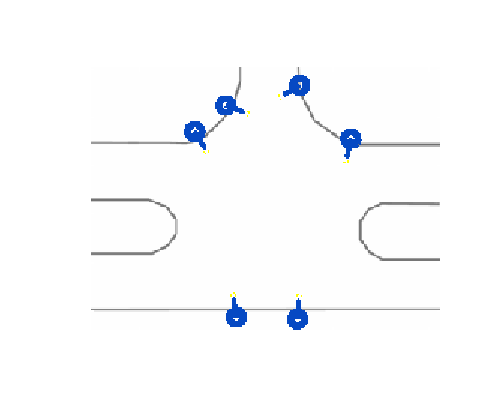
\includegraphics{fig/intersection_config-inc}
\end{picture}%
\begin{picture}(225,180)(0,0)
\fontsize{8}{0}
\selectfont\put(58.8969,24.856){\makebox(0,0)[t]{\textcolor[rgb]{0,0,0}{{-20}}}}
\fontsize{8}{0}
\selectfont\put(105.224,24.856){\makebox(0,0)[t]{\textcolor[rgb]{0,0,0}{{0}}}}
\fontsize{8}{0}
\selectfont\put(151.55,24.856){\makebox(0,0)[t]{\textcolor[rgb]{0,0,0}{{20}}}}
\fontsize{8}{0}
\selectfont\put(197.877,24.856){\makebox(0,0)[t]{\textcolor[rgb]{0,0,0}{{40}}}}
\fontsize{8}{0}
\selectfont\put(30,39.3877){\makebox(0,0)[r]{\textcolor[rgb]{0,0,0}{{-20}}}}
\fontsize{8}{0}
\selectfont\put(30,62.5511){\makebox(0,0)[r]{\textcolor[rgb]{0,0,0}{{-10}}}}
\fontsize{8}{0}
\selectfont\put(30,85.7144){\makebox(0,0)[r]{\textcolor[rgb]{0,0,0}{{0}}}}
\fontsize{8}{0}
\selectfont\put(30,108.878){\makebox(0,0)[r]{\textcolor[rgb]{0,0,0}{{10}}}}
\fontsize{8}{0}
\selectfont\put(30,132.041){\makebox(0,0)[r]{\textcolor[rgb]{0,0,0}{{20}}}}
\fontsize{8}{0}
\selectfont\put(30,155.204){\makebox(0,0)[r]{\textcolor[rgb]{0,0,0}{{30}}}}
\fontsize{8}{0}
\selectfont\put(119.307,11.856){\makebox(0,0)[t]{\textcolor[rgb]{0,0,0}{{x [m]}}}}
\fontsize{8}{0}
\selectfont\put(10,93.15){\rotatebox{90}{\makebox(0,0)[b]{\textcolor[rgb]{0,0,0}{{y [m]}}}}}
\fontsize{8}{0}
\selectfont\put(119.307,166.459){\makebox(0,0)[b]{\textcolor[rgb]{0,0,0}{{Intersection configuration}}}}
\fontsize{8}{0}
\selectfont\put(107.54,33.8285){\makebox(0,0)[l]{\textcolor[rgb]{0,0,0}{{ LMS1}}}}
\fontsize{8}{0}
\selectfont\put(136.911,33.041){\makebox(0,0)[l]{\textcolor[rgb]{0,0,0}{{ LMS5}}}}
\fontsize{8}{0}
\selectfont\put(162.437,124.166){\makebox(0,0)[l]{\textcolor[rgb]{0,0,0}{{ LMS2}}}}
\fontsize{8}{0}
\selectfont\put(137.93,149.877){\makebox(0,0)[l]{\textcolor[rgb]{0,0,0}{{ LMS3}}}}
\fontsize{8}{0}
\selectfont\put(90.8623,142.604){\makebox(0,0)[l]{\textcolor[rgb]{0,0,0}{{ LMS8}}}}
\fontsize{8}{0}
\selectfont\put(75.9915,129.956){\makebox(0,0)[l]{\textcolor[rgb]{0,0,0}{{ LMS7}}}}
\end{picture}

\caption{System setup}
\label{inter_cfg}
\end{figure}
 
\subsection{Preprocessing}

As mentioned before, the dataset provides a background model for each laser scanner. This model was generated using a histogram of each sampling angle of scanning, then a peak is found indicating a motionless object, considered as background. With the peak values at all sampling angles the background model is obtained. Now, when a new frame comes from the laser scanner, the measure at certain angle is compared with the peak value associated with that angle. If the difference is larger than a given threshold, the measured value is considered to belong to a moving object at the intersection. In figure \ref{bg_proc} is described the background removal process.



\begin{figure}[ht!]
\centering

% Title: glps_renderer figure
% Creator: GL2PS 1.3.8, (C) 1999-2012 C. Geuzaine
% For: Octave
% CreationDate: Mon Nov 23 08:06:36 2015
\setlength{\unitlength}{1pt}
\begin{picture}(0,0)
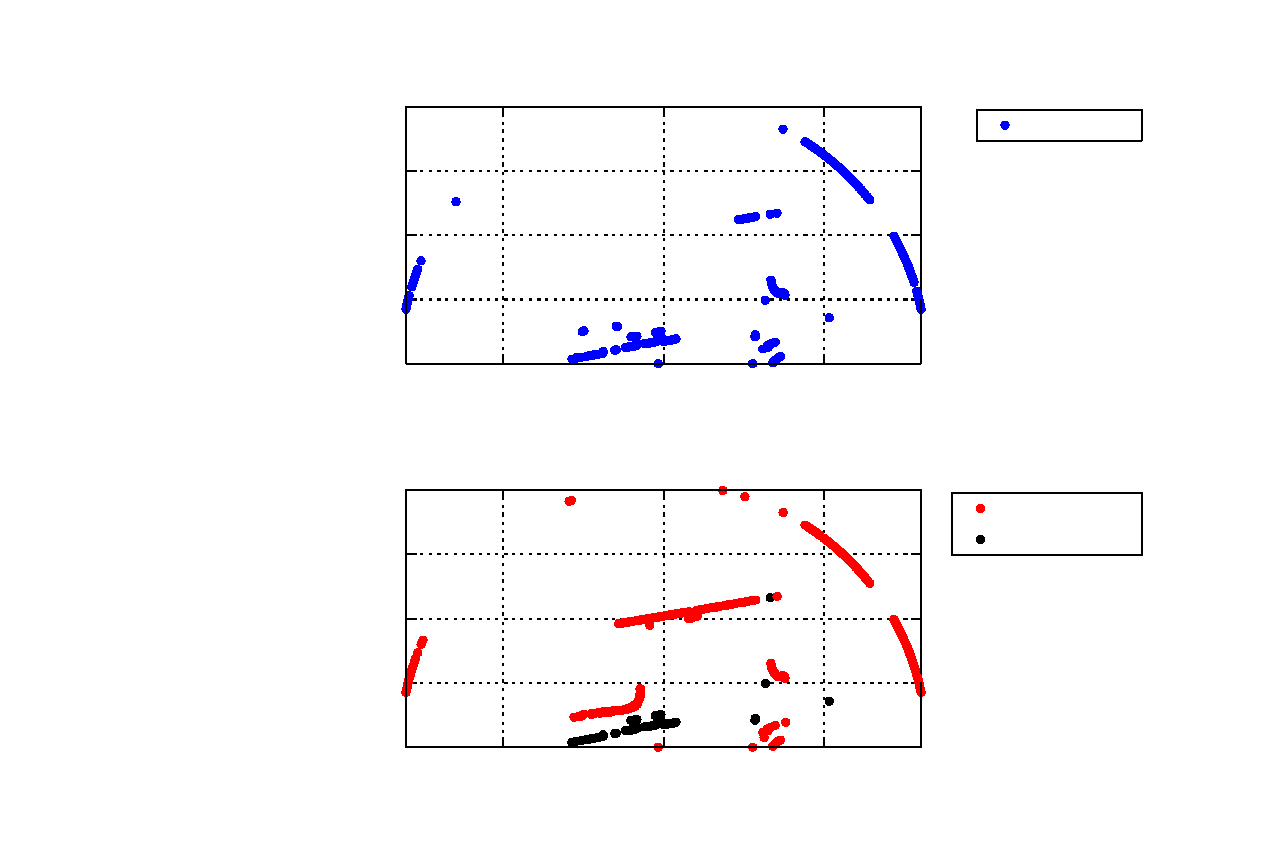
\includegraphics{fig/4/bg_process-inc}
\end{picture}%
\begin{picture}(600,400)(0,0)
\fontsize{10}{0}
\selectfont\put(233.334,228.516){\makebox(0,0)[t]{\textcolor[rgb]{0,0,0}{{-5000}}}}
\fontsize{10}{0}
\selectfont\put(310.5,228.516){\makebox(0,0)[t]{\textcolor[rgb]{0,0,0}{{0}}}}
\fontsize{10}{0}
\selectfont\put(387.666,228.516){\makebox(0,0)[t]{\textcolor[rgb]{0,0,0}{{5000}}}}
\fontsize{10}{0}
\selectfont\put(182.036,233.535){\makebox(0,0)[r]{\textcolor[rgb]{0,0,0}{{0}}}}
\fontsize{10}{0}
\selectfont\put(182.036,264.401){\makebox(0,0)[r]{\textcolor[rgb]{0,0,0}{{2000}}}}
\fontsize{10}{0}
\selectfont\put(182.036,295.267){\makebox(0,0)[r]{\textcolor[rgb]{0,0,0}{{4000}}}}
\fontsize{10}{0}
\selectfont\put(182.036,326.134){\makebox(0,0)[r]{\textcolor[rgb]{0,0,0}{{6000}}}}
\fontsize{10}{0}
\selectfont\put(182.036,357){\makebox(0,0)[r]{\textcolor[rgb]{0,0,0}{{8000}}}}
\fontsize{10}{0}
\selectfont\put(310.5,367){\makebox(0,0)[b]{\textcolor[rgb]{0,0,0}{{Raw laser data}}}}
\fontsize{10}{0}
\selectfont\put(488,348.095){\makebox(0,0)[l]{\textcolor[rgb]{0,0,0}{{Raw data}}}}
\fontsize{10}{0}
\selectfont\put(233.334,44.516){\makebox(0,0)[t]{\textcolor[rgb]{0,0,0}{{-5000}}}}
\fontsize{10}{0}
\selectfont\put(310.5,44.516){\makebox(0,0)[t]{\textcolor[rgb]{0,0,0}{{0}}}}
\fontsize{10}{0}
\selectfont\put(387.666,44.516){\makebox(0,0)[t]{\textcolor[rgb]{0,0,0}{{5000}}}}
\fontsize{10}{0}
\selectfont\put(182.036,49.5349){\makebox(0,0)[r]{\textcolor[rgb]{0,0,0}{{0}}}}
\fontsize{10}{0}
\selectfont\put(182.036,80.4012){\makebox(0,0)[r]{\textcolor[rgb]{0,0,0}{{2000}}}}
\fontsize{10}{0}
\selectfont\put(182.036,111.267){\makebox(0,0)[r]{\textcolor[rgb]{0,0,0}{{4000}}}}
\fontsize{10}{0}
\selectfont\put(182.036,142.134){\makebox(0,0)[r]{\textcolor[rgb]{0,0,0}{{6000}}}}
\fontsize{10}{0}
\selectfont\put(182.036,173){\makebox(0,0)[r]{\textcolor[rgb]{0,0,0}{{8000}}}}
\fontsize{10}{0}
\selectfont\put(310.5,183){\makebox(0,0)[b]{\textcolor[rgb]{0,0,0}{{Background model and extracted foreground}}}}
\fontsize{10}{0}
\selectfont\put(476.214,164.095){\makebox(0,0)[l]{\textcolor[rgb]{0,0,0}{{Background}}}}
\fontsize{10}{0}
\selectfont\put(476.214,149.175){\makebox(0,0)[l]{\textcolor[rgb]{0,0,0}{{Foreground}}}}
\end{picture}

\caption{Example of background removal applied to frame 123 from laser scanner 2 of dataset. In the upper plot, the raw data from the laser scanner is depicted. In the lower plot, red points represent the background model estimated based on peak values of the histogram. Black points are those marked as foreground after comparison of raw data with background data. The threshold used was 20. (Axis in centimeters).}
\label{bg_proc}
\end{figure}


\subsection{Feature Analysis}

Clustering is performed on the foreground extracted to identify the set of points belonging to the same object. The algorithm used in this implementation is DBSCAN, which stands for Density-Based Spatial Clustering of Applications with Noise. This algorithm does not need an estimated number of clusters as input, instead of this, it requires only two parameters: a minimum number of points per cluster, m, and a neighbourhood measure, $\epsilon$. A detailed description of the algorithm, can be found in \cite{Ester96}.

\subsection{Pattern Recognition}

At this stage, a bounding box is computed for each cluster found in previous stage. Them, the area and center of the bounding box are calculated and this is stored as a Blob entity. Now, blob information and scen model are analyzed in order to get more knowledge about how are blobs distributed over the legs of intersection.

\subsection{Situation Assesment}

-TODO-

\section{Results}

Three different scene configurations were defined in order to test the system proposal: using a single laser scanner, using three laser scanners and another with all the six laser scanners available in the dataset.


\subsection{Scene 1: Single laser scanner}

For this configuration laser scanner LMS2 is chosen because it has a good coverage of intersection and leg 2.

\subsection{Scene 2: Three laser scanners}

In this configuration selected laser scanners are LMS1, LMS2 and LMS3 trying to have a general coverage of the intersection from different views

\subsection{Scene 3: Six laser scanners}
This configuration uses all the available laser from the dataset.

\section{Conclusions and Future Work}

-TODO-

{\small
\bibliographystyle{unsrt}
\bibliography{../bibliography}
}

\end{document}